\documentclass[12pt]{article}
\usepackage[left=1cm, right=1cm, top=2cm,bottom=1.5cm]{geometry} 

\usepackage[parfill]{parskip}
\usepackage[utf8]{inputenc}
\usepackage[T2A]{fontenc}
\usepackage[russian]{babel}
\usepackage{enumitem}
\usepackage[normalem]{ulem}
\usepackage{amsfonts, amsmath, amsthm, amssymb, mathtools}
\usepackage{tikz}
\usepackage{tabularx}
\usepackage{hhline}

\usepackage{accents}
\usepackage{fancyhdr}
\pagestyle{fancy}
\renewcommand{\headrulewidth}{1.5pt}
\renewcommand{\footrulewidth}{1pt}

\usepackage{graphicx}
\usepackage[figurename=Рис.]{caption}
\usepackage{subcaption}
\usepackage{float}

%%Наименование папки откуда забирать изображения
\graphicspath{ {./images/} }

%%Изменение формата для ввода доказательства
\renewcommand{\proofname}{$\square$  \nopunct}
\renewcommand\qedsymbol{$\blacksquare$}

%%Изменение отступа на таблицах
\addto\captionsrussian{%
	\renewcommand{\proofname}{$\square$ \nopunct}%
}
%% Римские цифры
\newcommand{\RN}[1]{%
	\textup{\uppercase\expandafter{\romannumeral#1}}%
}

%% Для удобства записи
\newcommand{\MR}{\mathbb{R}}
\newcommand{\MQ}{\mathbb{Q}}
\newcommand{\MC}{\mathbb{C}}
\newcommand{\MI}{\mathrm{I}}
\newcommand{\MJ}{\mathrm{J}}
\newcommand{\MH}{\mathrm{H}}
\newcommand{\MT}{\mathrm{T}}
\newcommand{\MU}{\mathcal{U}}
\newcommand{\MV}{\mathcal{V}}
\newcommand{\VN}{\varnothing}
\newcommand{\VE}{\varepsilon}

\theoremstyle{definition}
\newtheorem{defn}{Опр:}
\newtheorem{rem}{Rm:}
\newtheorem{prop}{Утв.}
\newtheorem{exrc}{Упр.}
\newtheorem{lemma}{Лемма}
\newtheorem{theorem}{Теорема}
\newtheorem{corollary}{Следствие}

\newenvironment{cusdefn}[1]
{\renewcommand\thedefn{#1}\defn}
{\enddefn}

\DeclareRobustCommand{\divby}{%
	\mathrel{\text{\vbox{\baselineskip.65ex\lineskiplimit0pt\hbox{.}\hbox{.}\hbox{.}}}}%
}
%Короткий минус
\DeclareMathSymbol{\SMN}{\mathbin}{AMSa}{"39}
%Длинная шапка
\newcommand{\overbar}[1]{\mkern 1.5mu\overline{\mkern-1.5mu#1\mkern-1.5mu}\mkern 1.5mu}
%Функция знака
\DeclareMathOperator{\sgn}{sgn}

%Обозначение константы
\DeclareMathOperator{\const}{\text{const}}

%Интеграл в большом формате
\DeclareMathOperator{\dint}{\displaystyle\int}

\newcommand{\smallerrel}[1]{\mathrel{\mathpalette\smallerrelaux{#1}}}
\newcommand{\smallerrelaux}[2]{\raisebox{.1ex}{\scalebox{.75}{$#1#2$}}}

\newcommand{\smallin}{\smallerrel{\in}}
\newcommand{\smallnotin}{\smallerrel{\notin}}

\newcommand*{\medcap}{\mathbin{\scalebox{1.25}{\ensuremath{\cap}}}}%
\newcommand*{\medcup}{\mathbin{\scalebox{1.25}{\ensuremath{\cup}}}}%

%Скалярное произведение
\DeclarePairedDelimiterX{\inner}[2]{\langle}{\rangle}{#1, #2}

%Подпись символов снизу
\newcommand{\ubar}[1]{\underaccent{\bar}{#1}}

\newcommand*\circled[1]{\tikz[baseline=(char.base)]{
		\node[shape=circle,draw,inner sep=2pt] (char) {#1};}}

\begin{document}
\lhead{Линейная алгебра}
\chead{Мануйлов В.М.}
\rhead{Лекция - 1}

\textbf{Литература}
\begin{enumerate}[label={\arabic*)}]
	\item Гельфанд: Лекции по линейной алгебре;
	\item Кострикин и Манин: Линейная алгебра и геометрия;
\end{enumerate}

\section*{Линейные пространства}
\begin{enumerate}[label=\protect\circled{\arabic*}]
	\item Множество векторов плоскости или пространства;
	\item Строки или столбцы из $n$ чисел $(a_1, \dotsc, a_n)$;
	\item Числовые последовательности;
	\item Разные классы функций: $C(-\infty,\infty), \, C[0,1]$;
	\item Многочлены;
	\item Матрицы $n\times m$;
\end{enumerate}

\uwave{\textbf{Поле $\mathbb{K}$}}: элементы поля будем называть числами (скалярами), чаще всего полям это $\MR$ или $\MC$.

\begin{defn}
	\uwave{Линейным пространством} над полем $\mathbb{K}$ называется множество $V$ с операциями $+$ (сложение двух элементов из $V$) и $\cdot$ (умножение элемента из $V$ на скаляр), которые удовлетворяют свойствам:
	\begin{enumerate}[label={(\arabic*)}]
		\item в $V$ существует нулевой элемент $0 \in V \colon 0 + a = a, \, \forall a \in V$;
		\item $\forall a \in V, \exists \, b \in V \colon a + b = 0$;
		\item $a + b = b + a, \, \forall a,b \in V$;
		\item $(a + b) + c = a + (b + c), \, \forall a,b,c \in V$;
		\item $\lambda{\cdot}(a + b) = \lambda{\cdot}a + \lambda{\cdot}b, \, \forall \lambda \in \mathbb{K},\, \forall a,b \in V$;
		\item $(\lambda + \mu){\cdot}a = \lambda{\cdot}a + \mu{\cdot}a, \, \forall \lambda, \mu \in \mathbb{K},\, \forall a \in V$;
		\item $(\lambda{\cdot}\mu){\cdot}a = \lambda{\cdot}(\mu{\cdot}a), \, \forall \lambda, \mu \in \mathbb{K}, \, \forall a \in V$;
		\item $1{\cdot}a = a, \, \forall a \in V$;
	\end{enumerate}
\end{defn}

Если выполнены свойства $(1)-(4) \Rightarrow V$ - \uwave{абелева группа}.

\begin{corollary}\hfill
	\begin{enumerate}
		\item Единственность $0$;
		\begin{proof}
			Пусть $\exists \, 0, 0^\prime \in V$ - нули $\Rightarrow \forall a\in V,\, 0 + a = a, \, 0^\prime + a = a \Rightarrow 0^\prime = 0 + 0^\prime = 0^\prime + 0 = 0$.
		\end{proof}
		\item Единственность обратного элемента (обозначаем $-a$);
		\begin{proof}
			Пусть $\forall a, \exists \, b, b^\prime \in V \colon a + b = 0 \wedge a + b^\prime = 0 \Rightarrow b^\prime = b^\prime + 0 = b^\prime + (a + b) = (b^\prime + a) + b = 0 + b = b$.
		\end{proof}
		\item $0 \in \mathbb{K}, \, 0{\cdot}a = 0, \, \forall a \in V$;
		\begin{proof}
			$\forall a \in V \Rightarrow 0 = a + (-a) = 1{\cdot}a + (-a) = (1 + 0){\cdot}a +(-a) = 1{\cdot}a + 0{\cdot}a + (-a) = 0{\cdot}a + a + (-a) = $\\
			$= 0{\cdot}a + 0 = 0{\cdot}a$.
		\end{proof}
	\newpage
		\item $(-1){\cdot}a = -a, \, \forall a \in V$;
		\begin{proof}
			$\forall a \in V \Rightarrow 0 = 0{\cdot}a = (1-1){\cdot}a = 1{\cdot}a - 1{\cdot}a = a + (-1){\cdot}a = a + (-a) \Rightarrow (-1){\cdot}a = -a$.
		\end{proof}
	\end{enumerate}
\end{corollary}

\section*{Аффинные пространства}

\begin{defn}
	\uwave{Аффинное пространство} это набор $(\mathcal{A}, V, +)$  такой, что:
	\begin{enumerate}[label={(\arabic*)}]
		\item $P + 0 = P, \, \forall P \in \mathcal{A}, \, 0 \in V$;
		\item $(P + a) + b = P + (a + b), \, \forall P \in \mathcal{A},\, \forall a,b \in V,\, P + a \in \mathcal{A}$;
		\item $\forall P,Q \in \mathcal{A}, \exists! \, a \in V \colon P + a = Q$;
	\end{enumerate}
	где $\mathcal{A}$ это множество, $V$ это линейное пространство, $+$ это операция сложения: $P + v \in \mathcal{A}, \, P \in \mathcal{A}, \, v \in V$.
\end{defn}
\begin{figure}[H]
	\centering
	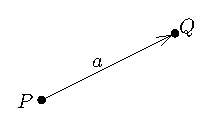
\includegraphics[width=0.2\textwidth]{1_1.eps}
	\caption{Сложение точки с вектором в аффинном пространстве.}
	\label{1_1}
\end{figure}
\begin{rem}
	\uline{Аффинное} $\Rightarrow$ \uline{линейное} (просто забудем про $\mathcal{A}$). \uline{Линейное} $\Rightarrow$ \uline{аффинное} ($V$ - линейное, $\mathcal{A} \vcentcolon= V$, $+$ это операция в $V$).
\end{rem}

\textbf{Пример}: $A$ - матрица, $X$ - столбец, $AX = 0$ - однородная СЛУ, $V$ - множество решений СЛУ,\\
$X_1, X_2$ - решения $\Rightarrow X_1 + X_2 \in V$, $\lambda{\cdot}X_1 \in V$, $\lambda{\cdot}X_2 \in V \Rightarrow$ \uline{линейное пространство}.

\textbf{Пример}: $AX = B$ - неоднородная СЛУ, не линейное пространство. Пусть $\mathcal{A}$ - множество решений,\\
$V$ - множество решений однородной СЛУ: $AX = 0$. Решение однородное $+$ решение неоднородное $=$ решение неоднородное $\Rightarrow$ \uline{аффинное пространство}.

\section*{Линейные подпространства}

\begin{defn}
	Пусть $V$ - линейное пространство над $\mathbb{K}$. Подмножество $L \subset V$ называется \uwave{линейным}\\ 
	\uwave{подпространством}, если $\forall a,b \in L, \, a + b \in L \wedge \forall \lambda \in \mathbb{K}, \, \forall a \in L, \, \lambda{\cdot}a \in L$.
\end{defn}

\textbf{Примеры}: $V$ - множество всех столбцов $\begin{pmatrix} x_1\\ \vdots\\x_n \end{pmatrix}$, $L \subset V, \, L$ - множество решений $Ax = 0 \Rightarrow$ \\
$V$ - линейное пространство, $L$ - линейное подпространство (для $Ax =B$ - не будет линейных подпространств). Тогда:
\begin{enumerate}[label={\arabic*)}]
	\item $L = \{0\}$ - линейное подпространство;
	\item $L = V$ - линейное подпространство;
	\item $a \neq 0,\, a\in V, \, L = \{\, \lambda{\cdot}a\colon \lambda \in \mathbb{K} \,\}$ - линейное подпространство;
\end{enumerate}

Пусть $a_1, \dotsc, a_n \in V$.
\begin{defn}
	\uwave{Линейной оболочкой} элементов $\{a_1, \dotsc, a_n\}$, где $a_i \in V$ называются всевозможные выражения вида $\lambda_1a_1 + \lambda_2 a_2 + \dotsc + \lambda_n a_n$, где $\lambda_1, \dotsc, \lambda_n \in \mathbb{K}$. Обозначение $\langle a_1, \dotsc, a_n\rangle$.
\end{defn}

\begin{lemma}
	Пусть $a_1, \dotsc, a_n \in V$, линейная оболочка $\langle a_1, \dotsc, a_n \rangle$ является линейным подпространством.
\end{lemma}
\begin{proof}
	Пусть $b,c \in \langle a_1, \dotsc, a_n \rangle, \, b = \lambda_1a_1 + \dotsc + \lambda_n a_n, \, c = \mu_1 a_1 + \dotsc + \mu_n a_n \Rightarrow$
	$$b + c = (\lambda_1 + \mu_1)a_1 + \dotsc (\lambda_n + \mu_n)a_n \in \langle a_1, \dotsc, a_n \rangle, \,  \alpha{\cdot}b = (\alpha \lambda_1)a_1 + \dotsc + (\alpha \lambda_n)a_n \in \langle a_1, \dotsc, a_n \rangle$$
	Таким образом получили линейное подпространство.
\end{proof}

\section*{Линейное подмногообразие}
\begin{defn}
	Пусть $a \in V,\, L \subset V$ - линейное подпространство. \uwave{Линейным подмногообразием} определенным по $a$ и $L$ называется множество $L_a = \{\, a + b \colon b \in L \,\}$.
\end{defn}

\textbf{Пример}: $L$ - подпространство $V$, $a \in V$, тогда $L_a$ представляется в следующем виде:
\begin{figure}[H]
	\centering
	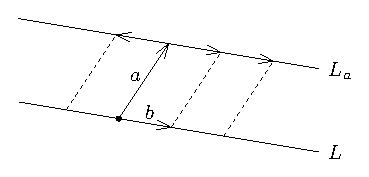
\includegraphics[width=0.35\textwidth]{1_2.eps}
	\caption{Линейное подмногообразие $L_a$.}
	\label{1_2}
\end{figure}

\textbf{Пример}: $AX = B$, $a$ - частное решение неоднородной системы, $L$ - множество решений однородной СЛУ, $L_a$ - множество всех решений неоднородной СЛУ.

Задаемся вопросом, когда $L_{a_1} = L_{a_2}$ - ?
\begin{lemma}
	$L_{a_1} = L_{a_2} \Leftrightarrow a_1 - a_2 \in L$.
\end{lemma}
\begin{proof}\hfill\\
	$(\Leftarrow)$ $a_1 - a_2 \in L \Rightarrow$ надо доказать, что $L_{a_1} \subset L_{a_2}$ (обратное включение получится по симметрии). $x \in L_{a_1} \Rightarrow$ $$\exists \, b \in L \colon x = a_1 + b = a_1 - a_2 + a_2 + b = a_2 + \underbrace{\overset{\in L}{(a_1 - a_2)} + \overset{\in L}{b}}_{\in L} = a_2 + b^\prime \in L_{a_2}$$ 
	где $b^\prime \in L$.
	
	$(\Rightarrow)$ $a_1 \in L_{a_1}$, так как $a_1 + 0 = a_1 \in L_{a_1}$. $L_{a_1} = L_{a_2} \Rightarrow a_2 + b \in L_{a_2}$, где $b \in L, \, a_1 \in L_{a_2} \Rightarrow$
	$$\exists \, b \in L \colon a_1 = a_2 + b \Rightarrow a_1 - a_2 = b \in L$$
\end{proof}

\newpage
\subsection*{Множество всех линейных подмногообразий $L_\alpha$}
Задано фиксированное $L$, берем всевозможные $a$ и получаем всевозможные $L_a$.
\begin{figure}[H]
	\centering
	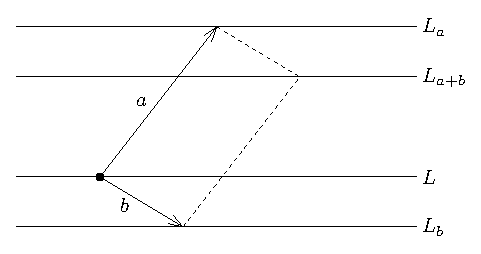
\includegraphics[width=0.45\textwidth]{1_3.eps}
	\caption{Составление нового линейного подмногообразия $L_{a + b}$.}
	\label{1_3}
\end{figure}
Введем структуру линейного пространства на этом множестве:
\begin{enumerate}[label={(\arabic*)}]
	\item $\forall a,b \in V, \, L_a + L_b = L_{a+b}$;
	\item $\forall a \in V, \, \forall \lambda \in \mathbb{K},\, \lambda{\cdot}L_a = L_{\lambda a}$;
\end{enumerate}
Проверим корректность: $L_a = L_{a^\prime}, \, L_b = L_{b^\prime}$ тогда.
\begin{enumerate}[label={(\arabic*)}]
	\item $L_{a+b} = L_{a^\prime + b^\prime}$;
	\begin{proof} 
			$a - a^\prime \in L, \, b - b^\prime \in L \Rightarrow a - a^\prime + b - b^\prime =(a+b) - (a^\prime + b^\prime) \in L \Rightarrow  L_{a+b} = L_{a^\prime + b^\prime}$. 
	\end{proof}
	\item $L_{\lambda a} = L_{\lambda a^\prime}$;
	\begin{proof}
		$a - a^\prime \in L \Rightarrow \lambda{\cdot}(a-a^\prime) \in L \Rightarrow \lambda{\cdot}a - \lambda{\cdot}a^\prime \in L \Rightarrow L_{\lambda a} = L_{\lambda a^\prime}$.
	\end{proof}
\end{enumerate}

\begin{defn}
	Множество всех линейных подмножеств, при фиксированном $L$ и $\forall a \in V$, удовлетворяющее условиям $(1)$ и $(2)$ называется \uwave{факторпространством} $V/L$.
\end{defn}

\begin{exrc}
	$L = \{0\}, \, L = V$, чему равно $V/L$?
\end{exrc}
\end{document}